%%%%%%%%%%%%%%%%%%%%%%%%%%%%%%%%%%%%%%%%%%%%%%%%%%%%%%%%%%%%%%%%%%%%%%%%%%%%%%%%
\section{Login To Mogon-NHR}
{   
	\usebackgroundtemplate{
		\vbox to \paperheight{\vfil\hbox to \paperwidth{\hfil\includegraphics[height=.7\paperheight]{misc/ssh.png}\hfil}\vfil}
	}
	\frame{
		\frametitle{How to log in to Remote Systems}
		\begin{mdframed}[tikzsetting={draw=white,fill=white,fill opacity=0.8,
				line width=0pt},backgroundcolor=none,leftmargin=0,
			rightmargin=150,innertopmargin=4pt,roundcorner=10pt]
			\tableofcontents[currentsection,sections={1-4},hideothersubsections]
		\end{mdframed} 
		\vspace{12mm}\hfill{\tiny \lhref{https://www.flaticon.com/de/kostenlose-icons/ssh"}{from Flavicon}}
	}
}

%%%%%%%%%%%%%%%%%%%%%%%%%%%%%%%%%%%%%%%%%%%%%%%%%%%%%%%%%%%%%%%%%%%%%%%%%%%%%%%%
\begin{frame}
	\frametitle{What is this about?}
	\begin{question}[Questions]
		\begin{itemize}
			\item How can log-in to Mogon-NHR?
			\item What is 2-Factor Authentication (2FA)?
		\end{itemize}
	\end{question}
	\begin{docs}[Objectives]
		\begin{enumerate}
			\item understanding 2FA basics
			\item being able to create and store ssh-keys
			\item being able to login in
		\end{enumerate}
	\end{docs}
\end{frame}

%%%%%%%%%%%%%%%%%%%%%%%%%%%%%%%%%%%%%%%%%%%%%%%%%%%%%%%%%%%%%%%%%%%%%%%%%%%%%%%%
\subsection{2FA}

%%%%%%%%%%%%%%%%%%%%%%%%%%%%%%%%%%%%%%%%%%%%%%%%%%%%%%%%%%%%%%%%%%%%%%%%%%%%%%%%
\begin{frame}
	\frametitle{2-Factor Authentication???}
	\begin{columns}
		\begin{column}{0.6\textwidth}
			\includegraphics[width=0.9\textwidth]{humor/2FA.jpg}
		\end{column}
		\begin{column}{0.4\textwidth}
			To ensure save logins, we use a 2-Factor Authentication Scheme:
			\begin{itemize}[<+->]
				\item The $1^\mathsf{st}$ factor is your account - or better a ssh-key associated with it.
				\item The $2^\mathsf{nd}$ factor is a device attributed to you - via a token on your mobile.
			\end{itemize}
			
		\end{column}
	\end{columns}
	
\end{frame}

%%%%%%%%%%%%%%%%%%%%%%%%%%%%%%%%%%%%%%%%%%%%%%%%%%%%%%%%%%%%%%%%%%%%%%%%%%%%%%%%
\subsection{ssh}

%%%%%%%%%%%%%%%%%%%%%%%%%%%%%%%%%%%%%%%%%%%%%%%%%%%%%%%%%%%%%%%%%%%%%%%%%%%%%%%%
\begin{frame}[fragile]
	\frametitle{Secure Shell (ssh)}
	\vspace{-1em}
	\begin{block}{What is \texttt{ssh}}
		\begin{quote}
			Secure Shell (SSH) is a cryptographic network protocol for operating network services securely over an unsecured network.
			Typical applications include remote command-line login and remote command execution, but any network service can be secured with SSH.
		\end{quote}
	\end{block}
	\pause
	The general command syntax is:
	\begin{lstlisting}[language=Bash, style=Shell,escapeinside={(*}{*)}]
$ ssh [options] [<user>(*@*)]<host>
	\end{lstlisting}
	\vspace{-1em}
	\begin{hint}
		If \altverb{<user>@} is ommitted \altverb{ssh} tries to login in on \altverb{host} with the current username.
	\end{hint}
\end{frame}

%%%%%%%%%%%%%%%%%%%%%%%%%%%%%%%%%%%%%%%%%%%%%%%%%%%%%%%%%%%%%%%%%%%%%%%%%%%%%%%%
\begin{frame}
	\frametitle{ssh-keys -- Why?}
	\begin{columns}[t]
		\begin{column}{.5\textwidth}
			\includegraphics[width=0.5\textwidth]{login/ssh_key.png}
			\begin{itemize}
				\item A ssh-key lets you log in to a known remote system without the need to re-type your password. (Just the passphrase -- occasionaly.)
				\item It may follow different encryption standards. Follow the advice of the remote provider or choose a default.
			\end{itemize}
		\end{column}
		\begin{column}{.5\textwidth}
			\begin{warning}
				Never publish your private key!
			\end{warning}
			\vfill
		\end{column}
	\end{columns}
\end{frame}

%%%%%%%%%%%%%%%%%%%%%%%%%%%%%%%%%%%%%%%%%%%%%%%%%%%%%%%%%%%%%%%%%%%%%%%%%%%%%%%%
\begin{frame}
	\frametitle{ssh-keys -- Best Practice?}
	\begin{exampleblock}{About Passphrases}
		\begin{itemize}[<+->]\footnotesize
			\item A passphrase is \emph{not} a password and should not be equal to any password.
			\item You may create more than one ssh-key.
			\item Best, use a password manager to store your passphrases.
		\end{itemize}
	\end{exampleblock}
	\pause[\thebeamerpauses]
	\begin{exampleblock}{How many Keys?}\footnotesize
		You can generate and register a number of keys (e.\,g. for your office, your remote location, your laptop, etc.). Or use a crypto stick to store \textbf{one} key along with passwords/passphrases.
	\end{exampleblock}
	\pause
	\begin{exampleblock}{Handling Keys and Passphrases}
		\begin{enumerate}\footnotesize
			\item Either you have a crypto stick (Yubi-key, Nitro-key, etc.) - then you need to transport your stick and remember one PIN.
			\item Or you best use a password manger (e.\,g. \lhref{https://keepass.info/download.html}{keepass (Windows, Linux) or keepass2 (Linux, OSX)} - Linux and OSX users may refer to their respective package managers.)
		\end{enumerate}
	\end{exampleblock}
\end{frame}

%%%%%%%%%%%%%%%%%%%%%%%%%%%%%%%%%%%%%%%%%%%%%%%%%%%%%%%%%%%%%%%%%%%%%%%%%%%%%%%%
\begin{frame}[fragile]
	\frametitle{\Interlude{Checking for existing keys}}
	You \emph{might} have a key registered already. This means, you \emph{might} have a key on Linux, too.\newline\pause
	\begin{task}
		Check whether you have an existing key with a standard name.
	\end{task}

	\begin{lstlisting}[language=Bash, style=Shell]
$ # Please run
$ ls ~/.ssh/id_ed25519
	\end{lstlisting}
	\pause
	\begin{columns}
		\begin{column}{0.7\textwidth}
			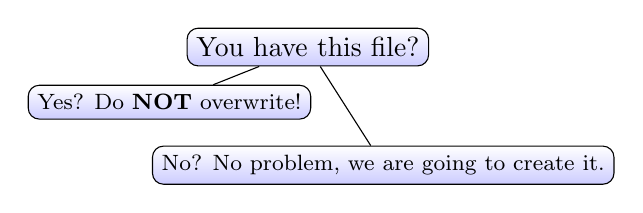
\begin{tikzpicture}[sibling distance=10em,
				every node/.style = {shape=rectangle, rounded corners,
					draw, align=center,
					top color=white, bottom color=blue!20}]]
				\node {You have this file?}
				child { node[yshift=+0.8cm] {\footnotesize Yes? Do \textbf{NOT} overwrite!} }
				child { node[xshift=-0.8cm] {\footnotesize No? No problem, we are going to create it.} };
			\end{tikzpicture}
		\end{column}
		\begin{column}{0.3\textwidth}
			\begin{task}
				Remember your result!
			\end{task}
		\end{column}
	\end{columns}	
	\vfill
\end{frame}


%%%%%%%%%%%%%%%%%%%%%%%%%%%%%%%%%%%%%%%%%%%%%%%%%%%%%%%%%%%%%%%%%%%%%%%%%%%%%%%% 
\begin{frame}[fragile]
	\frametitle{Preparing a ssh-key - Linux and OSX}
	In your terminal carry out:
	\begin{lstlisting}[language=Bash, style=Shell] 
$ ssh-keygen -a 256 -t ed25519 -C "HPCGATE,HPCLOGIN"
	\end{lstlisting}
    \begin{hint}
    	\footnotesize You will be asked, which prefix the key file should have and where it is saved, the default is \altverb{\~/.ssh/config/id_25519}. The public part will have a \altverb{.pub} suffix.
    \end{hint}

	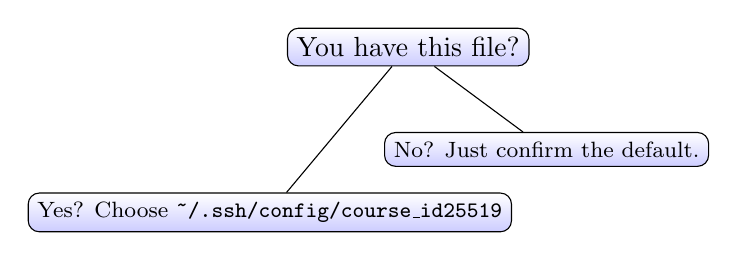
\begin{tikzpicture}[sibling distance=10em,
		every node/.style = {shape=rectangle, rounded corners,
			draw, align=center,
			top color=white, bottom color=blue!20}]]
		\node {You have this file?}
		child { node[yshift=-0.6cm] {\footnotesize Yes? Choose \texttt{\textasciitilde/.ssh/config/course\_id25519}} }
		child { node[yshift=0.2cm] {\footnotesize No? Just confirm the default.} };
	\end{tikzpicture}
\end{frame}


%%%%%%%%%%%%%%%%%%%%%%%%%%%%%%%%%%%%%%%%%%%%%%%%%%%%%%%%%%%%%%%%%%%%%%%%%%%%%%%% 
\begin{frame}
	\frametitle{Register your ssh-key with your Account}
	\begin{exampleblock}{Registering an ssh-key with the ZDV}
		You can take your ssh-key (e.\,g. from \texttt{\textasciitilde/.ssh/}) and navigate to \url{account.uni-mainz.de} and copy-paste the \texttt{public} part of your ssh-key, e.\,g. \texttt{\textasciitilde/.ssh/config/id\_ed25519.pub} .
	\end{exampleblock}
	\centering
	\includegraphics[width=0.8\textwidth]{login/adding_ssh_keys}
\end{frame}

%%%%%%%%%%%%%%%%%%%%%%%%%%%%%%%%%%%%%%%%%%%%%%%%%%%%%%%%%%%%%%%%%%%%%%%%%%%%%%%% 
\begin{frame}
	\frametitle{Login Options for Windows}
	We describe the basic login options in our wiki.\newline
	Basically there are three options:
	\begin{enumerate}
		\item via \lhref{https://www.putty.org/}{putty} -- a lightweight \texttt{ssh} implementation on Windows (see our \lhref{https://docs.hpc.uni-mainz.de/docs/getting-started/mogon-login/}{wiki})
		\item or \lhref{https://mobaxterm.mobatek.net/}{mobaxterm} -- free and commercial implementation of \texttt{ssh} on Windows (see our \lhref{https://docs.hpc.uni-mainz.de/docs/getting-started/mogon-login/}{wiki})
		\item or (since Windows 10) using the PowerShell (see our \lhref{https://docs.hpc.uni-mainz.de/docs/getting-started/mogon-login/}{wiki})
	\end{enumerate}
	Users of the Windows Subsystem for Linux (\lhref{https://en.wikipedia.org/wiki/Windows_Subsystem_for_Linux}{WSL}) are able to use \texttt{ssh} natively like Linux users.
	\vfill
\end{frame}

%%%%%%%%%%%%%%%%%%%%%%%%%%%%%%%%%%%%%%%%%%%%%%%%%%%%%%%%%%%%%%%%%%%%%%%%%%%%%%%% 
\begin{frame}
	\frametitle{Using Linux-Like Logins}
	\begin{docs}
		Except for \texttt{mobaxterm} and \texttt{putty} all other ssh implementations are like the Linux one:
		\begin{itemize}
			\item the \texttt{PowerShell} on Windows has the same look \& feel as on Linux
			\item OSX is a UNIX derivative, anyway. Except for the need to install X11 via \texttt{brew}, everything is the same as for Linux users.
			\item WSL users need admin priviledges to install WSL - ask your local OU admin, if you want to use WSL.
		\end{itemize}
	\end{docs}
	
	\pause
	\begin{hint}
		This is why we focus on Linux.
	\end{hint}
\end{frame}


%%%%%%%%%%%%%%%%%%%%%%%%%%%%%%%%%%%%%%%%%%%%%%%%%%%%%%%%%%%%%%%%%%%%%%%%%%%%%%%%
\begin{frame}[fragile]
	\frametitle{What is an ssh Configuration File?}
	All re-occuring settings can be put in a configuration file (Linux, only). The standard location is:
	\begin{lstlisting}[language=Bash, style=Shell] 
/home/<username>/.ssh/config 
	\end{lstlisting}
	\begin{columns}
		\begin{column}{.5\textwidth}
			A sample:
			\begin{lstlisting}[basicstyle=\tiny] 
# MOGON jump host
Host hpcgate
HostName hpcgate.zdv.uni-mainz.de
User <username>    
ForwardX11 yes    
IdentityFile ~/Path/To/Private/Key

# for access to MOGON NHR:
Host mogon-nhr
HostName mogon-nhr-01
User <username>
ProxyJump hpcgate    
ForwardX11 yes    
IdentityFile ~/Path/To/Private/Key
			\end{lstlisting}
		\end{column}
		\begin{column}{.5\textwidth}
			More \lhref{https://docs.hpc.uni-mainz.de/docs/getting-started/mogon-login/}{info is in our wiki}
			\begin{hint}
				\texttt{\textasciitilde/Path/To/Private/Key} is not necessary when using the default.
			\end{hint}
		\end{column}
	\end{columns} 
\end{frame}

%%%%%%%%%%%%%%%%%%%%%%%%%%%%%%%%%%%%%%%%%%%%%%%%%%%%%%%%%%%%%%%%%%%%%%%%%%%%%%%%
\begin{frame}[fragile]
	\frametitle{ssh Graphics Forwarding}
	When setting up your account you inevitably encountered a few options. An important one is the so-called ``\emph{X11 forwarding}'' -- the forwarding of graphical user interfaces.
	\pause
	\begin{exampleblock}{Linux and OSX users}
		Be sure to have a line reading 
		\begin{lstlisting}[language=Bash, style=Shell]
ForwardX11 yes
		\end{lstlisting}
		in your ssh configuration file.
	\end{exampleblock}
	\pause 
	\begin{exampleblock}{Windows Users}
		Windows users should enable the X11 option in their respective programs. See \lhref{https://docs.hpc.uni-mainz.de/docs/getting-started/mogon-login/}{our wiki} for more information.
	\end{exampleblock}
\end{frame}

%%%%%%%%%%%%%%%%%%%%%%%%%%%%%%%%%%%%%%%%%%%%%%%%%%%%%%%%%%%%%%%%%%%%%%%%%%%%%%%%
\begin{frame}[fragile]
	\frametitle{With and without a Configuration}
	Without a configuration file, a command line might look like:
	\begin{lstlisting}[style=Plain] 
$ ssh -i ~/Path/To/Private/Key \
> -J <username>@hpcgate.zdv.uni-mainz.de  \
> -i ~/Path/To/Private/Key <username>@mogon
	\end{lstlisting}
	\pause
	Or with a configuration file:
	\begin{lstlisting}[language=Bash, style=Shell]
$ ssh mogon-nhr
	\end{lstlisting}
\end{frame}

%%%%%%%%%%%%%%%%%%%%%%%%%%%%%%%%%%%%%%%%%%%%%%%%%%%%%%%%%%%%%%%%%%%%%%%%%%%%%%%%
\setcounter{handson}{\value{preframe_handson}}
\begin{frame}[fragile]
	\setcounter{preframe_handson}{\value{handson}}
	\frametitle{\HandsOn{Copy the Configuration File}}
	\begin{enumerate}[<+->]
		\item Using your browser, navigate to \url{https://docs.hpc.uni-mainz.de/docs/getting-started/connection-setup/#ssh-config} (you may search for ``\texttt{mogondocs}'', too.
		\item As ``\emph{\small Access MOGON from outside of the university network using UNIX} look for the configuration and copy \& paste it into an editor (e.\,g. \altverb{gedit}).
		\item Adjust ''\texttt{<username>}`` for your username.
		\item Save the file at \altverb{\~/.ssh/config}. As invisible folders are not listed, save as \altverb{config} first and then
		\begin{lstlisting}[language=Bash, style=Shell]
$ cat config >> ~/.ssh/config # >> appends to an existing file
		\end{lstlisting}
	\end{enumerate}
\end{frame}


%%%%%%%%%%%%%%%%%%%%%%%%%%%%%%%%%%%%%%%%%%%%%%%%%%%%%%%%%%%%%%%%%%%%%%%%%%%%%%%%
\begin{frame}<handout:0>
	\frametitle{Synchronization takes Time}
	\begin{hint}
		Now, that you registered your key, we either take a short break or postpone logging in.
	\end{hint}
\end{frame}


%%%%%%%%%%%%%%%%%%%%%%%%%%%%%%%%%%%%%%%%%%%%%%%%%%%%%%%%%%%%%%%%%%%%%%%%%%%%%%%%
\subsection{Login to Mogon}

%%%%%%%%%%%%%%%%%%%%%%%%%%%%%%%%%%%%%%%%%%%%%%%%%%%%%%%%%%%%%%%%%%%%%%%%%%%%%%%%
\begin{frame}<handout:0>
	\frametitle{It is now time to log in}
	If not already done, now is the time to log to the "Mogon-NHR" cluster.\\
\end{frame}

%%%%%%%%%%%%%%%%%%%%%%%%%%%%%%%%%%%%%%%%%%%%%%%%%%%%%%%%%%%%%%%%%%%%%%%%%%%%%%%% 
\begin{frame}[fragile]
	\frametitle{Logging In}
	Login via Linux or OSX is \lhref{https://mogonwiki.zdv.uni-mainz.de/dokuwiki/start:mogon_cluster:access_from_outside_unix}{described in the wiki, too}. Once an ssh configuration file is adapted, the command line becomes:
	\begin{lstlisting}[language=Bash, style=Shell,escapeinside={(*}{*)}]
$ ssh mogon-nhr
	\end{lstlisting}
    \begin{task}
    	Please, carry out this command - you will be asked to confirm, that your really want to log-in (type "yes"). Next, you will be asked for your one-time-password.
    \end{task}
\end{frame}


%%%%%%%%%%%%%%%%%%%%%%%%%%%%%%%%%%%%%%%%%%%%%%%%%%%%%%%%%%%%%%%%%%%%%%%%%%%%%%%%
\begin{frame}<handout:0>[fragile]
	\frametitle{Testing Graphics Forwarding}
	You can now test whether the X11-forwarding has been sucessfully enabled. The following line will start a new terminal in the background:
	\begin{lstlisting}[language=Bash, style=Shell]
$ xterm &
	\end{lstlisting}
    You may just close the mini-terminal.
\end{frame}

%%%%%%%%%%%%%%%%%%%%%%%%%%%%%%%%%%%%%%%%%%%%%%%%%%%%%%%%%%%%%%%%%%%%%%%%%%%%%%%%
\subsection*{Policies}

%%%%%%%%%%%%%%%%%%%%%%%%%%%%%%%%%%%%%%%%%%%%%%%%%%%%%%%%%%%%%%%%%%%%%%%%%%%%%%%%
\setcounter{interlude}{\value{preframe_interlude}}
\begin{frame}[fragile]
	\setcounter{preframe_interlude}{\value{interlude}}
	\frametitle{\Interlude{Policies}}
	Now, that you are logged in: Behave yourself! Remember that you are not alone on the system.
	\pause
	\begin{block}{Doubts?}
		Just type \verb+who+ and you will believe us.
	\end{block}
	\pause
	\begin{alertblock}{Login Nodes}
		The purpose of login nodes is to arrange your data and submit jobs (content of the HPC intro course). Please refrain from doing actual jobs on login nodes. However, it is o.\,k. to perform brief tests ($\ll$ 1\,h), even in parallel (few cores).
	\end{alertblock}
\end{frame}
